\chapter{التعقيد}\label{ch:b1:complexation}

اسكب قليلًا من محلول الأمونيا في كبريتات النحاس(II) الزرقاء الباهتة: يتكوّن
في الحال راسب أزرق باهت. واسكب المزيد، فيذوب الراسب
في محلول أزرق قاتم يكاد يكون بلون الحبر. ولا شيء في فصلي
الحمض--القاعدة والترسيب يفسّر الخطوة الثانية. فقد ارتبطت
جزيئات الأمونيا بأيون النحاس عبر أزواجها الحرة
وكوّنت نوعًا جديدًا، هو \omterm{def:b1:complexation:complex}{معقد}، أكثر استقرارًا من الهيدروكسيد ومختلفًا
عنه لونًا. \omterm{def:b1:complexation:complex}{فالمعقدات} تحمل الأكسجين في الدم، وتمسك الفلز
في اليخضور وفي الفيتامين \babelsublr{B$_{12}$}، وتيسّر الماء العسر وتذيب
فلزات لا يذيبها شيء آخر. ويعاملها هذا الفصل على أنها تبادل آخر
للجسيمات في الماء، له ثوابته ومخططاته الخاصة.

\begin{recall}
عُرّفت أحماض لويس (مستقبلات أزواج الإلكترونات) وقواعد لويس (مانحات أزواج الإلكترونات)
\omterm{def:b1:lewis-resonance-vsepr:lewis-acid}{والرابطة التناسقية} في \cref{ch:b1:lewis-resonance-vsepr}.
ومصدر \omterm{def:b1:predominant-reaction:predominance}{مخططات الغلبة} وطريقة \omterm{def:b1:predominant-reaction:predominant-reaction}{التفاعل الغالب}
\cref{ch:b1:predominant-reaction}؛ ومصدر \omterm{def:b1:precipitation:solubility-product}{جداء الذوبانية}
وشرط الترسيب \cref{ch:b1:precipitation}.
\end{recall}

\begin{omfigure}
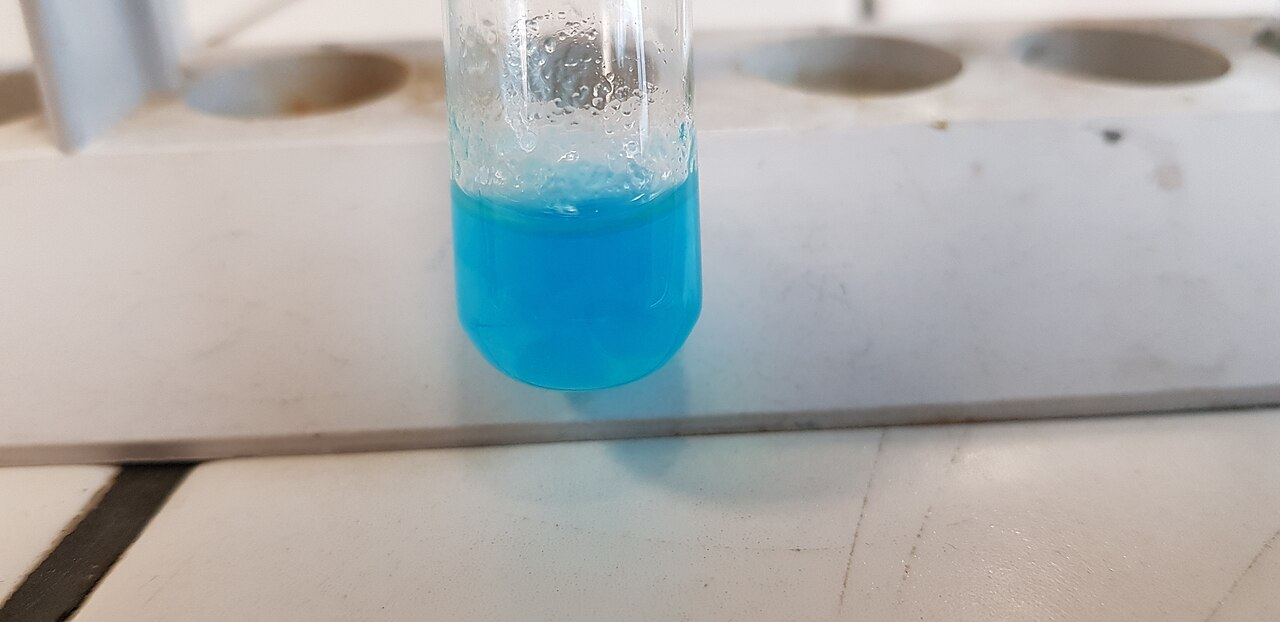
\includegraphics[height=4.2cm]{images/book2/copper-hydroxide.jpg}\hspace{0.6em}%
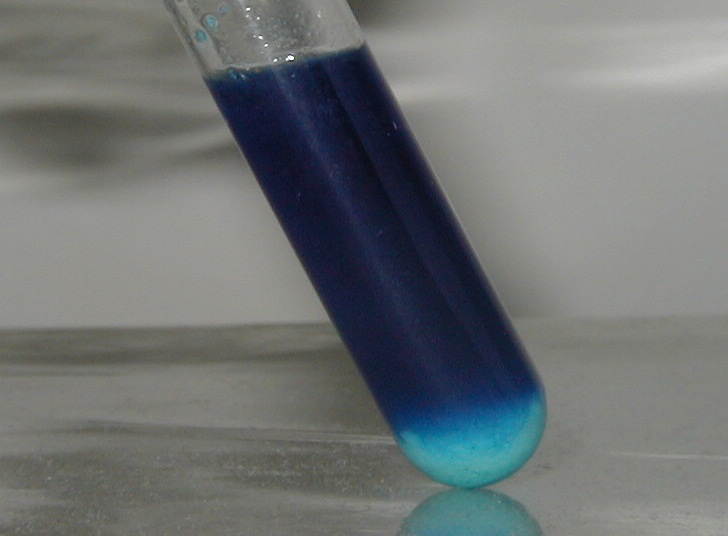
\includegraphics[height=4.2cm]{images/book2/copper-ammine.jpg}

{\small يمينًا: معلّق من هيدروكسيد النحاس(II) الأزرق الباهت
(تصوير ألفي16، CC BY 4.0). يسارًا: مع مزيد من الأمونيا يذوب الجسم الصلب
في أيون رباعي أمين النحاس(II) الأزرق القاتم؛ ولا يزال بعض الهيدروكسيد غير
المذاب في قعر الأنبوب (تصوير كيميكال إنترست،
ملكية عامة). كلتاهما من ويكيميديا كومنز.}
\end{omfigure}

\section{المعقدات والربائط}

\begin{definition}[المعقد، الذرة المركزية، الربيطة]\label{def:b1:complexation:complex}
\emph{المعقد}\index{معقد} نوع كيميائي مكوّن من \emph{ذرة
مركزية}\index{ذرة مركزية} أو أيون مركزي، هو عادةً كاتيون فلزي يسلك سلوك
\omterm{def:b1:lewis-resonance-vsepr:lewis-acid}{حمض لويس}، مرتبط بروابط تناسقية بجزيئات أو أيونات تسلك سلوك قواعد
لويس، هي \emph{الربائط}\index{ربيطة}. وتُكتب صيغته بين
معقوفين، مع شحنته الكلية: $[\ce{Cu(NH3)4}]^{2+}$،
$[\ce{Fe(CN)6}]^{4-}$، $[\ce{Ag(NH3)2}]^{+}$، $[\ce{FeSCN}]^{2+}$.
\end{definition}

شحنة \omterm{def:b1:complexation:complex}{المعقد} هي مجموع شحنة الأيون المركزي
وشحنات \omterm{def:b1:complexation:complex}{الربائط}: فالأيون $\mathrm{Fe^{2+}}$ وستة أيونات \ce{CN-} تكوّن
$[\ce{Fe(CN)6}]^{4-}$. وتحتاج \omterm{def:b1:complexation:complex}{الربيطة} إلى \omterm{def:b1:lewis-resonance-vsepr:lewis}{زوج حر} واحد على الأقل: \ce{NH3}،
\ce{H2O}، \ce{OH-}، \ce{Cl-}، \ce{CN-}، \ce{SCN-} (مرتبطًا عبر S أو N).
وكل أيون فلزي في الماء هو في الواقع \omterm{def:b1:complexation:complex}{معقد} أصلًا مع جزيئات الماء
ربائطَ، $[\ce{Cu(H2O)6}]^{2+}$ أو $[\ce{Fe(H2O)6}]^{3+}$؛
وتكوين \omterm{def:b1:complexation:complex}{معقد} آخر يعني استبدال ربائط أخرى بجزيئات الماء هذه،
وتُحذف ربائط الماء من الصيغ، كما يُكتب \ce{H3O+}
للبروتون المميَّه.

\begin{omfigure}
\begin{tikzpicture}[font=\small, line cap=round]
  % [Ag(NH3)2]+ : linear
  \begin{scope}
    \node (ag) at (0,0) {\ce{Ag}};
    \node (n1) at (-1.2,0) {\ce{H3N}};
    \node (n2) at (1.2,0) {\ce{NH3}};
    \draw[thick] (n1) -- (ag) -- (n2);
    \node at (0,-1.75) {\foreignlanguage{arabic}{$[\ce{Ag(NH3)2}]^{+}$، خطي}};
  \end{scope}
  % [Cu(NH3)4]2+ : square plane in perspective
  \begin{scope}[xshift=4.3cm, every node/.style={fill=white, inner sep=1.5pt}]
    \node (cu) at (0,0) {\ce{Cu}};
    \node (a) at (-1.45,-0.5) {\ce{H3N}};
    \node (b) at (1.45,0.5) {\ce{NH3}};
    \node (c) at (0.85,-0.9) {\ce{NH3}};
    \node (d) at (-0.85,0.9) {\ce{H3N}};
    \begin{pgfonlayer}{background}
    \draw[gray, dashed] (a.center) -- (c.center) -- (b.center) -- (d.center) -- cycle;
    \end{pgfonlayer}
    \draw[thick] (cu) -- (a); \draw[thick] (cu) -- (b);
    \draw[thick] (cu) -- (c); \draw[thick] (cu) -- (d);
    \node at (0,-1.75) {\foreignlanguage{arabic}{$[\ce{Cu(NH3)4}]^{2+}$، مربع مستوٍ}};
  \end{scope}
  % [Fe(CN)6]4- : octahedron
  \begin{scope}[xshift=9.2cm, every node/.style={fill=white, inner sep=1.5pt}]
    \node (fe) at (0,0) {\ce{Fe}};
    \node (t) at (0,1.3) {\ce{CN}};
    \node (u) at (0,-1.3) {\ce{CN}};
    \node (l) at (-1.45,-0.45) {\ce{NC}};
    \node (r) at (1.45,0.45) {\ce{CN}};
    \node (f) at (0.8,-0.8) {\ce{CN}};
    \node (k) at (-0.8,0.8) {\ce{NC}};
    \begin{pgfonlayer}{background}
    \draw[gray, dashed] (l.center) -- (f.center) -- (r.center) -- (k.center) -- cycle;
    \end{pgfonlayer}
    \foreach \x in {t,u,l,r,f,k} \draw[thick] (fe) -- (\x);
    \node at (0,-1.75) {\foreignlanguage{arabic}{$[\ce{Fe(CN)6}]^{4-}$، ثماني الأوجه}};
  \end{scope}
\end{tikzpicture}

{\small ثلاثة \omterm{def:b1:complexation:complex}{معقدات} وأشكالها. كل خط \omterm{def:b1:lewis-resonance-vsepr:lewis-acid}{رابطة تناسقية} من
\omterm{def:b1:lewis-resonance-vsepr:lewis}{الزوج الحر} \omterm{def:b1:complexation:complex}{للربيطة} (ذرة N في الأمونيا، وذرة C في السيانيد) إلى
الأيون الفلزي؛ والخطوط المتقطعة تحدد مربع \omterm{def:b1:complexation:complex}{الربائط} الأربع. وتُفسَّر أشكال
\omterm{def:b1:complexation:complex}{المعقدات} في مجلد السنة الثانية.}
\end{omfigure}

\begin{definition}[الربيطة المتعددة المخالب، المعقد المخلبي]\label{def:b1:complexation:chelate}
\omterm{def:b1:complexation:complex}{الربيطة} التي ترتبط بالأيون المركزي نفسه عبر عدة ذرات من ذراتها في
آن واحد \emph{ربيطة متعددة المخالب}\index{ربيطة متعددة المخالب}؛
\omterm{def:b1:complexation:complex}{والمعقد} الذي تكوّنه، والذي تُغلق فيه \omterm{def:b1:complexation:complex}{الربيطة} حلقات حول الأيون الفلزي،
\emph{معقد مخلبي}\index{معقد مخلبي}. فالإيثيلين ثنائي الأمين
\ce{H2N-CH2-CH2-NH2} يرتبط عبر ذرتي N، وأيون الأكسالات
\ce{C2O4^2-} عبر ذرتي O، وأيون الإيثيلين ثنائي الأمين رباعي الأسيتات
(\emph{الإديتا}، ويُكتب \ce{Y^4-}) عبر ذرتي N وأربع ذرات O.
\end{definition}

\begin{omfigure}
\setchemfig{atom sep=1.9em}
\chemfig{N(-[3]-[2]C(=[1]O)-[3]O^{-})(-[5]-[6]C(=[7]O)-[5]O^{-})-[0]-[0]N(-[1]-[2]C(=[3]O)-[1]O^{-})(-[7]-[6]C(=[5]O)-[7]O^{-})}
\hspace{2.2em}
\begin{tikzpicture}[font=\small, baseline=(ca.base)]
  \node[circle, draw, thick, fill=omDef!12, inner sep=1.5pt] (ca) at (0,0) {\ce{Ca}};
  \node (n1) at (-1.15,-0.35) {N};
  \node (n2) at (0.55,-0.6) {N};
  \node (o1) at (0,1.35) {O};
  \node (o2) at (0,-1.35) {O};
  \node (o3) at (1.15,0.35) {O};
  \node (o4) at (-0.55,0.6) {O};
  \foreach \x in {n1,n2,o1,o2,o3,o4} \draw[thick, omDef] (ca) -- (\x);
  \draw[omProp, thick] (n1) .. controls (-0.57,-0.95) .. (n2);
  \draw[omProp, thick] (n1) .. controls (-1.05,0.95) .. (o1);
  \draw[omProp, thick] (n1) .. controls (-1.5,0.25) .. (o4);
  \draw[omProp, thick] (n2) .. controls (0.5,-1.6) .. (o2);
  \draw[omProp, thick] (n2) .. controls (1.5,-0.3) .. (o3);
\end{tikzpicture}

{\small يمينًا: أيون الإديتا \ce{Y^4-}، بذرتي N وأربع
مجموعات كربوكسيلات. يسارًا: \omterm{def:b1:complexation:chelate}{المعقد المخلبي} كالسيوم--إديتا $[\ce{CaY}]^{2-}$،
رسمًا تخطيطيًا: تقع ذرات الإعطاء الست (الروابط الزرقاء) على رؤوس ثماني
أوجه حول الأيون، وذرتا N متجاورتان، وتُغلق سلاسل
الكربون في \omterm{def:b1:complexation:complex}{الربيطة} (بالبرتقالي) خمس حلقات خماسية الذرات، هي
الحلقات المخلبية.}
\end{omfigure}

يمسك أيون الإديتا أيون الكالسيوم بقوة تكفي ليكون كاشف
معايرة عسر الماء (\cref{ch:b1:titration-methods}).

\section{ثوابت التكوين والتفكك}

\begin{definition}[ثوابت التكوين والتفكك]\label{def:b1:complexation:formation-constant}
من أجل أيون مركزي M \omterm{def:b1:complexation:complex}{وربيطة} L (مع حذف الشحنات)، يكون \emph{ثابت
التكوين الإجمالي}\index{ثابت التكوين الإجمالي} \omterm{def:b1:complexation:complex}{للمعقد}
$\mathrm{ML}_n$ هو الثابت $\beta_n$ للتفاعل
$\mathrm{M} + n\,\mathrm{L} \rightleftharpoons \mathrm{ML}_n$،
\[
  \beta_n = \frac{[\mathrm{ML}_n]}{[\mathrm{M}][\mathrm{L}]^n} .
\]
و\emph{ثابت التكوين المتتالي}\index{ثابت التكوين المتتالي}
$K_i$ هو ثابت إضافة \omterm{def:b1:complexation:complex}{ربيطة} واحدة،
$\mathrm{ML}_{i-1} + \mathrm{L} \rightleftharpoons \mathrm{ML}_i$.
و\emph{ثابت التفكك}\index{ثابت التفكك} هو
مقلوبه، $K_d = 1/K_i$، و$\mathrm{p}K_d = \log K_i$، بحيث توصف
المزدوجة \omterm{def:b1:complexation:complex}{معقد}/\omterm{def:b1:complexation:complex}{ربيطة} تمامًا كما توصف مزدوجة حمض--قاعدة، مع
\omterm{def:b1:complexation:complex}{الربيطة} مكان البروتون.
\end{definition}

\begin{proposition}[الثوابت الإجمالية والمتتالية]\label{prop:b1:complexation:beta-k}
$\beta_n = K_1 K_2 \cdots K_n$، أي
$\log\beta_n = \sum_{i=1}^n \log K_i$ و$\log K_i = \log\beta_i -
\log\beta_{i-1}$ (مع $\beta_0 = 1$).
\end{proposition}

\begin{proof}
تكوين $\mathrm{ML}_n$ من M هو مجموع الإضافات المتتالية
$n$؛ وثابت مجموع تفاعلات هو جداء
ثوابتها (\cref{ch:b1:extent-q-and-k}). ومباشرة:
$K_1 K_2\cdots K_n = \frac{[\mathrm{ML}]}{[\mathrm{M}][\mathrm{L}]}
\frac{[\mathrm{ML_2}]}{[\mathrm{ML}][\mathrm{L}]}\cdots
\frac{[\mathrm{ML}_n]}{[\mathrm{ML}_{n-1}][\mathrm{L}]}$، فتُختصر
التراكيز الوسيطة.
\end{proof}

\begin{omfigure}
\begin{tabular}{lll}
\hline
\omterm{def:b1:complexation:complex}{المعقد} & $\log\beta_n$ & $\log K_i$ \\
\hline
$[\ce{Cu(NH3)_n}]^{2+}$، $n = 1$ إلى 4 & 4.10، 7.51، 10.33، 12.36 & 4.10، 3.41، 2.82، 2.03 \\
$[\ce{Ag(NH3)_n}]^{+}$، $n = 1, 2$ & 3.32، 7.22 & 3.32، 3.90 \\
$[\ce{Zn(OH)4}]^{2-}$ & $\log\beta_4 = 14.45$ & \\
$[\ce{FeSCN}]^{2+}$، $[\ce{FeF}]^{2+}$ & 2.96؛ 6.85 & \\
$[\ce{CaY}]^{2-}$، $[\ce{MgY}]^{2-}$، $[\ce{NiY}]^{2-}$ & 12.69، 10.90، 20.54 & \\
\hline
\end{tabular}

\smallskip
{\small ثوابت التكوين عند \qty{25}{\celsius}. ثوابت الأمين
والهيدروكسو والثيوسيانات والفلورو محسوبة من طاقات غيبس القياسية
المجدولة للتكوين؛ وثوابت الإديتا قيم منتقاة نقديًا
عند شدة أيونية معدومة، وكذلك قيم $\mathrm{p}K_a$ للإديتا المستعملة
أدناه، 2.23 و3.15 و6.80 و11.24.}
% ledger: dfg:Cu2+_ao, dfg:CuNH32+_ao, dfg:Cu_NH322+_ao, dfg:Cu_NH332+_ao, dfg:Cu_NH342+_ao, dfg:NH3_ao (computed in figdata/bachelor-1/aqueous-constants.py)
% ledger: dfg:Ag+_ao, dfg:AgNH3+_ao, dfg:Ag_NH32+_ao, dfg:Fe3+_ao, dfg:SCN-_ao, dfg:FeSCN2+_ao, dfg:F-_ao, dfg:FeF2+_ao (computed, same script)
% ledger: logb:Ca-edta, logb:Mg-edta, logb:Ni-edta, pka:edta1, pka:edta2, pka:edta3, pka:edta4
\end{omfigure}

تتناقص الثوابت المتتالية لأمينات النحاس، $K_1 > K_2 > K_3
> K_4$: فكل جزيء أمونيا يضاف يترك مواقع أقل ويجعل
\omterm{def:b1:complexation:complex}{المعقد} أقل إقبالًا قليلًا على الجزيء التالي. وهذا هو الترتيب المعتاد.
أما الفضة فاستثناء: $K_2 > K_1$، وتُستخلص نتائج ذلك في
مسألة نهاية الأسبوع.

\section{الغلبة بدلالة pL}

\begin{definition}[سلّم pL]\label{def:b1:complexation:pl-diagram}
من أجل \omterm{def:b1:complexation:complex}{ربيطة} L، $\mathrm{pL} = -\log[\mathrm{L}]$، حيث $[\mathrm{L}]$
تركيز \omterm{def:b1:complexation:complex}{الربيطة} الحرة. و\emph{سلّم pL}\index{سلم pL}
محور pL تُرسم عليه مناطق غلبة الأيون المركزي
ومعقداته، كما تُرسم مناطق الأحماض والقواعد
على محور pH.
\end{definition}

\begin{proposition}[الحدود على سلّم pL]\label{prop:b1:complexation:pl-boundaries}
من أجل المزدوجة $\mathrm{ML}_i/\mathrm{ML}_{i-1}$،
\[
  \mathrm{pL} = \log K_i + \log\frac{[\mathrm{ML}_{i-1}]}{[\mathrm{ML}_i]} ,
\]
فيغلب $\mathrm{ML}_{i-1}$ من أجل $\mathrm{pL} > \log K_i$
و$\mathrm{ML}_i$ من أجل $\mathrm{pL} < \log K_i$. وحين تتناقص $\log K_i$
مع $i$، يكون المخطط متتالية من المناطق: $\mathrm{ML}_n$ عند pL
الصغير (\omterm{def:b1:complexation:complex}{ربيطة} كثيرة)، ثم $\mathrm{ML}_{n-1}$، وهكذا حتى M عند pL الكبير.
\end{proposition}

\begin{proof}
نأخذ لوغاريتم $K_i = [\mathrm{ML}_i]/([\mathrm{ML}_{i-1}][\mathrm{L}])$:
$\log K_i = \log\frac{[\mathrm{ML}_i]}{[\mathrm{ML}_{i-1}]} + \mathrm{pL}$.
يتساوى الشكلان عند $\mathrm{pL} = \log K_i$، وتتغير النسبة
بعامل عشرة لكل وحدة pL. وتقع منطقة $\mathrm{ML}_i$ بين
$\log K_{i+1}$ و$\log K_i$، ولا توجد إلا إذا كان $\log K_{i+1} < \log
K_i$.
\end{proof}

\begin{method}[رسم مخطط pL]\label{met:b1:complexation:pl-diagram}
\begin{enumerate}
  \item انطلاقًا من قيم $\log\beta_n$، احسب قيم $\log K_i$ المتتالية.
  \item إن كانت متناقصة، فضع كلًّا منها عند حدها على محور pL:
        \omterm{def:b1:complexation:complex}{المعقد} الأغنى \omterm{def:b1:complexation:complex}{بالربائط} على اليسار (pL صغير)، والأيون
        الحر على اليمين.
  \item إذا كان $\log K_{i+1} > \log K_i$ لبعض القيم، فليس \omterm{def:b1:complexation:complex}{للمعقد} $\mathrm{ML}_i$
        منطقة: فهو يتفاعل مع نفسه معطيًا $\mathrm{ML}_{i-1}$
        و$\mathrm{ML}_{i+1}$. احذفه وارسم حدًا واحدًا بين
        $\mathrm{ML}_{i-1}$ و$\mathrm{ML}_{i+1}$ عند
        $\frac12(\log K_i + \log K_{i+1})$.
\end{enumerate}
\end{method}

\begin{omfigure}
\begin{tikzpicture}
\begin{axis}[
  width=0.78\linewidth, height=5.2cm, xmin=0, xmax=7, ymin=0, ymax=1.05,
  axis x line=bottom, axis y line=left, xlabel={\babelsublr{$\mathrm{pNH_3}$}},
  ylabel={كسر النحاس},
  tick label style={font=\small}, label style={font=\small}]
\addplot[omThm, thick] table[x=pL, y=M] {figdata/out/bachelor-1-ammine-distribution-copper.dat};
\addplot[omProp, thick] table[x=pL, y=ML] {figdata/out/bachelor-1-ammine-distribution-copper.dat};
\addplot[omMeth, thick] table[x=pL, y=ML2] {figdata/out/bachelor-1-ammine-distribution-copper.dat};
\addplot[black!60, thick] table[x=pL, y=ML3] {figdata/out/bachelor-1-ammine-distribution-copper.dat};
\addplot[omDef, very thick] table[x=pL, y=ML4] {figdata/out/bachelor-1-ammine-distribution-copper.dat};
\node[omDef, font=\small, anchor=west] at (axis cs:0.15,0.78) {$n = 4$};
\node[black!60, font=\small] at (axis cs:2.42,0.63) {3};
\node[omMeth, font=\small] at (axis cs:3.12,0.55) {2};
\node[omProp, font=\small] at (axis cs:3.76,0.58) {1};
\node[omThm, font=\small, anchor=east] at (axis cs:6.9,0.84) {\ce{Cu^2+}};
\end{axis}
\end{tikzpicture}

\begin{tikzpicture}[font=\small, x=1.25cm]
  \draw[->, thick] (0,0) -- (7.2,0) node[right] {$\mathrm{pNH_3}$};
  \foreach \x/\l in {2.03/2.03, 2.82/2.82, 3.41/3.41, 4.10/4.10}
    \draw (\x,0.12) -- (\x,-0.12) node[below] {\l};
  \node[above] at (1.0,0.08) {$[\ce{Cu(NH3)4}]^{2+}$};
  \node[above, font=\scriptsize] at (2.42,0.08) {3};
  \node[above, font=\scriptsize] at (3.12,0.08) {2};
  \node[above, font=\scriptsize] at (3.76,0.08) {1};
  \node[above] at (5.6,0.08) {\ce{Cu^2+}};
  \begin{scope}[yshift=-1.25cm]
  \draw[->, thick] (0,0) -- (7.2,0) node[right] {$\mathrm{pNH_3}$};
  \draw (3.61,0.12) -- (3.61,-0.12) node[below] {3.61};
  \draw[dotted] (3.32,0.3) -- (3.32,-0.1); \draw[dotted] (3.90,0.3) -- (3.90,-0.1);
  \node[above] at (1.6,0.08) {$[\ce{Ag(NH3)2}]^{+}$};
  \node[above] at (5.4,0.08) {\ce{Ag+}};
  \end{scope}
\end{tikzpicture}

{\small في الأعلى: كسور النحاس(II) الموجودة على هيئة \ce{Cu^2+}
و$[\ce{Cu(NH3)_n}]^{2+}$ ($n = 1$ إلى 4) بدلالة $\mathrm{pNH_3}$. في الوسط:
\omterm{def:b1:predominant-reaction:predominance}{مخطط غلبة} أمينات النحاس، وحدوده عند قيم
$\log K_i$. في الأسفل: الفضة، حيث $\log K_2 = 3.90 > \log K_1 = 3.32$
(بالنقاط): فليس \omterm{def:b1:complexation:complex}{للمعقد} $[\ce{AgNH3}]^{+}$ منطقة ويقع حد وحيد عند
$\frac12\log\beta_2 = 3.61$.}
\end{omfigure}

\begin{example}[النحاس في أمونيا تركيزها \texorpdfstring{\qty{0.010}{mol/L}}{0.010 mol/L}]\label{ex:b1:complexation:cu}
عند $[\ce{NH3}] = \qty{0.010}{mol/L}$ للأمونيا الحرة، يقع $\mathrm{pNH_3} = 2.0$ في
منطقة $[\ce{Cu(NH3)3}]^{2+}$ لكن قرب الحد 2.03 مع
$[\ce{Cu(NH3)4}]^{2+}$: فالاثنان متساويان تقريبًا. والكسور
متناسبة مع $\beta_n[\ce{NH3}]^n = 10^{\log\beta_n - 2n}$، أي
$1 : 10^{2.10} : 10^{3.51} : 10^{4.33} : 10^{4.36}$، فيكون \qty{48}{\percent} من
$[\ce{Cu(NH3)4}]^{2+}$، و\qty{45}{\percent} من $[\ce{Cu(NH3)3}]^{2+}$،
و\qty{7}{\percent} من $[\ce{Cu(NH3)2}]^{2+}$ ولا يكاد يوجد \ce{Cu^2+} حر.
\end{example}

\section{التنافسات}

يمكن أن يتنازع أيونان فلزيان ربيطةً، وربيطتان أيونًا فلزيًا،
وكلاهما منخرط أيضًا في توازنات الترسيب والحمض--القاعدة.
وكل تنافس تفاعل إضافي يجمع ثابته
الثوابت المعروفة أصلًا؛ ثم تنطبق طريقة \omterm{def:b1:predominant-reaction:predominant-reaction}{التفاعل الغالب} في
\cref{ch:b1:predominant-reaction} دون تغيير.

\begin{example}[ربيطتان للحديد \babelsublr{(III)}]\label{ex:b1:complexation:scn-f}
تعطي قطرة من الثيوسيانات في محلول حديد(III) \omterm{def:b1:complexation:complex}{المعقد} الأحمر الدموي
$[\ce{FeSCN}]^{2+}$؛ وتزيل أيونات الفلوريد لونه:
\[
  [\ce{FeSCN}]^{2+} + \ce{F-} \rightleftharpoons [\ce{FeF}]^{2+} + \ce{SCN-},
  \qquad K = \frac{\beta(\ce{FeF})}{\beta(\ce{FeSCN})} = 10^{6.85 - 2.96} =
  10^{3.89} .
\]
\omterm{def:b1:complexation:complex}{فالمعقد} الأقوى ($\beta$ الأكبر) يأخذ الأيون الفلزي، تمامًا كما يعطي
الحمض الأقوى بروتونه للقاعدة الأقوى.
\end{example}

\begin{proposition}[التعقيد في مواجهة الترسيب]\label{prop:b1:complexation:competition-precipitation}
يذوب الجسم الصلب MX في \omterm{def:b1:complexation:complex}{الربيطة} L وفق
$\mathrm{MX(s)} + n\,\mathrm{L} \rightleftharpoons \mathrm{ML}_n + \mathrm{X}$،
الذي ثابته $K = \beta_n K_s$. وإذا كان \omterm{def:b1:complexation:complex}{المعقد} هو الشكل الوحيد للعنصر M في
المحلول وكان تركيز \omterm{def:b1:complexation:complex}{الربيطة} الحرة $[\mathrm{L}]$، كانت
\omterm{def:b1:precipitation:solubility}{الذوبانية} $s = \sqrt{K}\,[\mathrm{L}]^{n/2}$.
\end{proposition}

\begin{proof}
التفاعل هو مجموع الذوبان (الثابت $K_s$)
وتكوين $\mathrm{ML}_n$ ($\beta_n$). وعند الإشباع $[\mathrm{ML}_n]
= [\mathrm{X}] = s$ و$K = s^2/[\mathrm{L}]^n$.
\end{proof}

\begin{method}[إذابة راسب بالتعقيد]\label{met:b1:complexation:dissolve-precipitate}
\begin{enumerate}
  \item اكتب تفاعل الذوبان إلى \omterm{def:b1:complexation:complex}{المعقد} واحسب
        $K = \beta_n K_s$.
  \item إذا كان $K$ كبيرًا، كان الذوبان \omterm{def:b1:extent-q-and-k:quantitative}{كمّيًا} ما دام
        في الوسط ما يكفي من \omterm{def:b1:complexation:complex}{الربيطة}؛ وإذا كان صغيرًا، فاحسب تركيز \omterm{def:b1:complexation:complex}{الربيطة} الحرة
        اللازم لذوبان كمية الجسم الصلب:
        $[\mathrm{L}]^n = s^2/K$.
  \item أضف \omterm{def:b1:complexation:complex}{الربيطة} المرتبطة في \omterm{def:b1:complexation:complex}{المعقد}، $n s$، لتحصل على
        الكمية الكلية من \omterm{def:b1:complexation:complex}{الربيطة} الواجب إدخالها.
  \item تحقق من أن الأيون الفلزي الحر مهمل: $[\mathrm{M}] = K_s/s
        \ll s$.
\end{enumerate}
\end{method}

مع الأمونيا، يذوب كلوريد الفضة ($K = 10^{7.22 - 9.75} = 10^{-2.53}$)
في محلول متوسط التركيز بينما لا يذوب يوديد الفضة
($K = 10^{-8.85}$): وتستعمل مسألة نهاية الأسبوع ذلك للتمييز بين
الهاليدات.

\begin{proposition}[التعقيد في مواجهة الحمضية]\label{prop:b1:complexation:ligand-acidity}
إذا كانت \omterm{def:b1:complexation:complex}{الربيطة} قاعدة $\mathrm{L}$ لحمض $\mathrm{HL}$ (و
ربما لأشكال أكثر برتنة)، فلا يتاح إلا الكسر $[\mathrm{L}]/c_L =
1/\alpha$ من \omterm{def:b1:complexation:complex}{الربيطة} غير المرتبطة بالفلز، مع
\[
  \alpha = 1 + \frac{[\ce{H3O+}]}{K_{an}} + \frac{[\ce{H3O+}]^2}{K_{an}K_{a(n-1)}}
  + \cdots
\]
($K_{an}$ \omterm{def:b1:predominant-reaction:acidity-constant}{ثابت الحمضية} الأخير). وعند pH ثابت يسلك التعقيد عندئذ
سلوك تفاعل ثابته هو الثابت \emph{المشروط}
$\beta' = \beta/\alpha$، الذي يصغر كلما انخفض pH.
\end{proposition}

\begin{proof}
تتوزع \omterm{def:b1:complexation:complex}{الربيطة} غير المرتبطة بالفلز بين L وHL و\ce{H2L}
وما بعدها، مع $[\mathrm{HL}] = [\mathrm{L}][\ce{H3O+}]/K_{an}$ وعلاقات
مماثلة للأشكال التالية (\cref{ch:b1:predominant-reaction}). وبالجمع نحصل على $c_L = \alpha[\mathrm{L}]$،
و$\beta = [\mathrm{ML}]/([\mathrm{M}][\mathrm{L}]) =
\alpha[\mathrm{ML}]/([\mathrm{M}]c_L)$، فيكون $[\mathrm{ML}]/([\mathrm{M}]c_L)
= \beta/\alpha$.
\end{proof}

ومن أجل الإديتا عند pH 10، $\alpha = 1 + 10^{11.24 - 10} + 10^{11.24 + 6.80 - 20}
= 18.4$، فيحتفظ \omterm{def:b1:complexation:complex}{معقد} الكالسيوم بالقيمة $\log\beta' = 12.69 - 1.26 = 11.43$؛
وعند pH 7 تهبط إلى 8.24 (\cref{exo:b1:complexation:9}). ولهذا
تُجرى معايرة الكالسيوم بالإديتا في \omterm{def:b1:predominant-reaction:buffer}{محلول منظم} أمونياكي عند pH 10.
والأمونيا أيضًا قاعدة: ففي الحمض تصير \ce{NH4+}، الذي لا \omterm{def:b1:lewis-resonance-vsepr:lewis}{زوج حر}
له، فتتفكك \omterm{def:b1:complexation:complex}{معقدات} الأمين. وإضافة حمض النتريك إلى
$[\ce{Ag(NH3)2}]^{+}$ في وجود الكلوريد تعيد الراسب
الأبيض لكلوريد الفضة.

ومثبّتات التصوير الفوتوغرافي تفعل الشيء نفسه \omterm{def:b1:complexation:complex}{بربيطة} أخرى لأيون الفضة،
هي أيون الثيوكبريتات \ce{S2O3^2-}: فهي تذيب هاليد الفضة الذي لم
يمسّه الضوء، كي لا تعود الصورة تسودّ. وثوابته
ليست من معطيات هذا المجلد؛ والأمونيا تُظهر الكيمياء نفسها
مع كلوريد الفضة.

\section{تمارين}

\begin{exercise}[$\star$]\label{exo:b1:complexation:1}
أعطِ لكل \omterm{def:b1:complexation:complex}{معقد} الأيون المركزي، وشحنته، \omterm{def:b1:complexation:complex}{والربائط}،
والذرة التي ترتبط عبرها كل \omterm{def:b1:complexation:complex}{ربيطة}: $[\ce{Cu(NH3)4}]^{2+}$،
$[\ce{Fe(CN)6}]^{4-}$، $[\ce{Fe(CN)6}]^{3-}$، $[\ce{Ag(NH3)2}]^{+}$،
$[\ce{FeSCN}]^{2+}$، $[\ce{Zn(OH)4}]^{2-}$، $[\ce{CaY}]^{2-}$.
\end{exercise}

\begin{exercise}[$\star$]\label{exo:b1:complexation:2}
انطلاقًا من قيم $\log\beta_n$ لأمينات النحاس، احسب قيم $\log K_i$ الأربع
وقيم $\mathrm{p}K_d$ الأربع. واكتب تفاعل التفكك الذي
تشير إليه قيمة $\mathrm{p}K_d$ الأخيرة.
\end{exercise}

\begin{exercise}[$\star$]\label{exo:b1:complexation:3}
ارسم مخطط pL لأمينات النحاس. أي نوع من أنواع النحاس
يغلب عند $[\ce{NH3}] = 1.0$ و\num{3.2e-3} و\num{3.2e-4}
و\qty{1.0e-5}{mol/L}؟
\end{exercise}

\begin{exercise}[$\star$]\label{exo:b1:complexation:4}
يحوي محلول الحديد(III) بتركيز \qty{1.0e-3}{mol/L} والثيوسيانات بتركيز
\qty{0.10}{mol/L}. بإهمال الثيوسيانات المرتبطة، ما الكسر من
الحديد الموجود على هيئة $[\ce{FeSCN}]^{2+}$؟
\end{exercise}

\begin{exercise}[$\star\star$]\label{exo:b1:complexation:5}
برهن على أنه في محلول لأيون فلزي M ومعقداته
$\mathrm{ML}_n$، يكون كسر $\mathrm{ML}_n$ هو
$\beta_n[\mathrm{L}]^n / \sum_{k} \beta_k[\mathrm{L}]^k$. وبيّن أنه،
إذا لم يوجد بكميات معتبرة إلا $\mathrm{ML}_{i-1}$ و$\mathrm{ML}_i$ و$\mathrm{ML}_{i+1}$،
كان كسر $\mathrm{ML}_i$ أكبر ما يكون حيث $[\mathrm{ML}_{i-1}] = [\mathrm{ML}_{i+1}]$، عند
$\mathrm{pL} = \frac12(\log K_i + \log K_{i+1})$، واحسب قيمة pNH3 هذه
\omterm{def:b1:complexation:complex}{للمعقد} $[\ce{Cu(NH3)2}]^{2+}$.
\end{exercise}

\begin{exercise}[$\star\star$]\label{exo:b1:complexation:6}
يضاف فلوريد الصوديوم إلى المحلول الأحمر في \cref{exo:b1:complexation:4}
حتى يصير $[\ce{F-}] = \qty{0.010}{mol/L}$ (حرًا). احسب ثابت
تبادل \omterm{def:b1:complexation:complex}{الربائط} والنسبة $[\ce{FeF^2+}]/[\ce{FeSCN^2+}]$.
ماذا يُرى؟
\end{exercise}

\begin{exercise}[$\star\star$]\label{exo:b1:complexation:7}
تضاف أيونات الكالسيوم إلى محلول $[\ce{MgY}]^{2-}$، بكمية
مساوية. اكتب تفاعل التبادل، واحسب ثابته
وكسر المغنيسيوم المحرَّر.
\end{exercise}

\begin{exercise}[$\star\star$]\label{exo:b1:complexation:8}
أكسيد الفضة \ce{Ag2O} جسم صلب بني: للتفاعل \ce{Ag2O(s) + H2O <=> 2Ag+ + 2OH-}
القيمة $\mathrm{p}K = 15.43$. اكتب ذوبانه في الأمونيا إلى
$[\ce{Ag(NH3)2}]^{+}$، واحسب الثابت، وفسّر لماذا يذوب الراسب
البني المتكوّن بقليل من الأمونيا في نترات الفضة في
مزيد من الأمونيا.
\end{exercise}

\begin{exercise}[$\star\star$]\label{exo:b1:complexation:9}
احسب $\alpha$ والثابت المشروط $\log\beta'$ \omterm{def:b1:complexation:complex}{للمعقد} $[\ce{CaY}]^{2-}$
عند pH 10 وعند pH 7 (\cref{prop:b1:complexation:ligand-acidity}). ولماذا
تستحيل معايرة الكالسيوم بالإديتا في محلول متعادل إذا كان
الثابت المشروط المطلوب $10^{10}$ على الأقل؟
\end{exercise}

\begin{exercise}[$\star\star\star$]\label{exo:b1:complexation:10}
أكسيد النحاس(II) \ce{CuO} هو الجسم الصلب الذي يتحول إليه هيدروكسيد النحاس(II)
مع الوقت؛ وللتفاعل \ce{CuO(s) + H2O <=> Cu^2+ + 2OH-} القيمة $\mathrm{p}K = 20.64$.
\begin{enumerate}
  \item اكتب ذوبان \ce{CuO} في الأمونيا إلى
        $[\ce{Cu(NH3)4}]^{2+}$ واحسب ثابته.
  \item في أمونيا تركيزها \qty{1.0}{mol/L} وحدها، تحدد الأمونيا
        \babelsublr{pH ($\mathrm{p}K_a(\ce{NH4+}) = 9.25$)}. احسب pH
        وتركيز النحاس المذاب.
  \item السؤال نفسه في \omterm{def:b1:predominant-reaction:buffer}{محلول منظم} من الأمونيا وكلوريد الأمونيوم، كلاهما
        بتركيز \qty{1.0}{mol/L}. استنتج.
\end{enumerate}
\end{exercise}

\begin{exercise}[$\star\star\star$]\label{exo:b1:complexation:11}
الفضة والأمونيا.
\begin{enumerate}
  \item بيّن أن $[\ce{AgNH3}]^{+}$ يتفاعل مع نفسه،
        \ce{2[AgNH3]+ <=> Ag+ + [Ag(NH3)2]+}، واحسب الثابت.
  \item احسب أكبر كسر من الفضة يوجد في أي وقت على هيئة
        $[\ce{AgNH3}]^{+}$، وقيمة pNH3 التي يحدث عندها.
\end{enumerate}
\end{exercise}

\begin{exercise}[$\star\star\star$]\label{exo:b1:complexation:12}
يُستعمل محلول إديتا، \qty{0.10}{mol/L} من \ce{Y^4-} عند pH مرتفع، لإذابة
ترسبات كربونات الكالسيوم.
\begin{enumerate}
  \item اكتب التفاعل واحسب ثابته.
  \item ما كتلة كربونات الكالسيوم التي يستطيع لتر واحد أن يذيبها؟
  \item لماذا يجب أن يكون المحلول قاعديًا؟ (أيونا الكربونات والإديتا
        كلاهما قاعدتان.)
\end{enumerate}
\end{exercise}

\section{مسألة: الأمونيا وهاليدات الفضة الثلاثة}

\begin{problem}[{مسألة نهاية الأسبوع --- أمينات الفضة وثوابتها
المعكوسة، وإذابة كلوريد الفضة وبروميدها ويوديدها في
الأمونيا، والاختبار التأكيدي، وأقل كمية من الأمونيا تذيب
غرامًا واحدًا من كلوريد الفضة}]
\label{pb:b1:complexation:1}
لدى محللة ثلاثة رواسب بين الأبيض والأصفر وعليها أن تقول أيها
كلوريد الفضة وأيها بروميدها وأيها يوديدها؛ ثم عليها أن
تذيب \qty{1.0}{g} من كلوريد الفضة في \qty{1.00}{L} بأقل
كمية ممكنة من الأمونيا. معطيات عند \qty{25}{\celsius}: $\log\beta_1 = 3.32$
و$\log\beta_2 = 7.22$ لأمينات الفضة؛ $\mathrm{p}K_s$ للمركب \ce{AgCl}
9.75، و\ce{AgBr} 12.27، و\ce{AgI} 16.07؛ $\mathrm{p}K_a(\ce{NH4+}) = 9.25$؛
والكتل المولية \ce{AgCl} \qty{143.4}{g/mol}، \ce{AgBr} \qty{187.8}{g/mol}،
\ce{AgI} \qty{234.8}{g/mol}.

\medskip
\noindent\textbf{الجزء الأول --- أمينات الفضة.}
\begin{enumerate}
  \item اكتب تفاعلي تكوين $[\ce{AgNH3}]^{+}$
        و$[\ce{Ag(NH3)2}]^{+}$ وعبارتي $\beta_1$ و$\beta_2$.
  \item احسب $\log K_1$ و$\log K_2$.
  \item ارسم مخطط pL بسذاجة بهذين الحدين. ما الخطأ
        فيه؟
  \item اكتب تفاعل $[\ce{AgNH3}]^{+}$ مع نفسه واحسب
        ثابته.
  \item ارسم المخطط الصحيح؛ أين يقع حده الوحيد؟
  \item عند $[\ce{NH3}] = \qty{0.10}{mol/L}$، احسب
        $[\ce{Ag(NH3)2+}]/[\ce{Ag+}]$.
  \item أعطِ \omterm{def:b1:complexation:formation-constant}{ثابت التفكك} الإجمالي $\mathrm{p}K_d$ \omterm{def:b1:complexation:complex}{للمعقد}
        $[\ce{Ag(NH3)2}]^{+}$.
\end{enumerate}

\medskip
\noindent\textbf{الجزء الثاني --- كلوريد الفضة في الأمونيا.}
\begin{enumerate}[resume]
  \item اكتب ذوبان \ce{AgCl} في الأمونيا واحسب
        ثابته.
  \item عبّر عن \omterm{def:b1:precipitation:solubility}{الذوبانية} $s$ دالةً في تركيز الأمونيا الحرة
        واحسبها من أجل $[\ce{NH3}] = \qty{1.0}{mol/L}$.
  \item بكم ازدادت \omterm{def:b1:precipitation:solubility}{الذوبانية} مقارنةً بالماء
        النقي؟
  \item ما كتلة كلوريد الفضة التي يذيبها لتر واحد عندئذ؟
  \item تحقق من أن \ce{Ag+} الحر مهمل.
  \item لنعدّ الآن \qty{1.0}{mol/L} الكمية الكلية من الأمونيا المُدخلة. مع
        مراعاة الأمونيا المرتبطة، احسب $s$ من جديد.
  \item الأمونيا قاعدة؛ فسّر لماذا يمكن إهمال برتنتها في
        هذا المحلول.
\end{enumerate}

\medskip
\noindent\textbf{الجزء الثالث --- البروميد واليوديد.}
\begin{enumerate}[resume]
  \item احسب ثابت ذوبان \ce{AgBr} في الأمونيا.
  \item احسب \omterm{def:b1:precipitation:solubility}{ذوبانية} \ce{AgBr} في أمونيا حرة تركيزها \qty{1.0}{mol/L}،
        بالوحدة \unit{mol/L} وبالوحدة \unit{g/L}.
  \item الأمر نفسه للمركب \ce{AgI}، بالوحدة \unit{mg/L}.
  \item استنتج طريقة للتعرف على الرواسب الثلاثة.
  \item ما تركيز الأمونيا الحرة الذي يذيب \qty{1.0}{g} من
        \ce{AgBr} في \qty{1.00}{L}؟
  \item الأمر نفسه من أجل \qty{1.0}{g} من \ce{AgI}. علّق.
\end{enumerate}

\medskip
\noindent\textbf{الجزء الرابع --- غرام واحد من كلوريد الفضة.}
\begin{enumerate}[resume]
  \item يضاف حمض النتريك إلى المحلول الأمونياكي لكلوريد الفضة.
        اكتب التفاعل الإجمالي واحسب ثابته. ماذا
        ترى المحللة؟
  \item ما تركيز الأمونيا الحرة اللازم لإذابة \qty{1.0}{g}
        من \ce{AgCl} في \qty{1.00}{L}؟
  \item كم من الأمونيا مرتبط في \omterm{def:b1:complexation:complex}{المعقد}؟
  \item تحقق من أن \ce{Ag+} الحر مهمل في هذا المحلول.
  \item ما أقل تركيز كلي للأمونيا يذيب
        \qty{1.0}{g} من كلوريد الفضة في \qty{1.00}{L}؟
\end{enumerate}
\end{problem}
